\documentclass[12pt,a4paper]{article}
\usepackage[utf8]{inputenc}
\usepackage{hyperref}
\usepackage{amssymb}
\usepackage{amsmath}
\usepackage{graphicx}
\usepackage{caption}
\usepackage{listings}
\captionsetup[figure]{labelfont={bf},name={Fig.},labelsep=period}
\captionsetup[table]{labelfont={bf},name={Tab.},labelsep=period}
\usepackage{multicol}
\usepackage{booktabs, makecell, longtable}

\title{Intervijas uzdevumi LVĢMC datu analītiķa pozīcijai}
% \title{Intervijas uzdevumi LV\c{G}MC datu anal\={\i}ti\c{k}a poz\={\i}cijai}
\author{Anete Valnere}
\date{\today}
\begin{document}

\begingroup
\let\center\flushright
\let\endcenter\endflushright
\maketitle
\endgroup
% \maketitle
% \big{Anete Valnere}
\section*{Pirmais uzdevums}


\begin{figure}[h]
    \centering
    \includegraphics[width=7cm]{kastes_kluda.png}
    \caption{Kastu grafiki pa stacijām}
\end{figure}
Pirmajā figūrā redzami kastu grafiki stacijās \(x_1\), \(x_2\) un \(x_3\). Uzreiz ir skaidrs, ka trešajā stacijā daži mērījumi nav pareizi, jo dati atšķiras par vairākām magnitūdām no abām pārējām stacijām.% Lai par to pārliecinātos, izvadīsim visus trešās stacijas datus, kas ir lielāki par pirmās un otrās stacijas maksimālajiem mērījumiem.


Apskatot datus trešajā stacijā, kuri ir lielāki par maksimālajām vērtībām pirmajā un otrajā stacijā, varam ievērot, ka visi šie mērījumi ir veikti devītajā jūlijā secīgās minūtēs, kā arī tie neseko skaidram rakstam, līdz ar to izteiksim pieņēmumu, ka vainīga ir sensora kļūda.

Pēc šo datu pārvēršanas par \texttt{NA} varam vēlreiz apskatīt kastu grafikus.

\noindent\begin{minipage}[t]{.7\textwidth}
    \centering
    \includegraphics[height=7cm]{kastes_labs.png}
    \captionof{figure}{Kastu grafiki pa stacijām}
\end{minipage}%
\begin{minipage}[t]{.3\textwidth}
    \centering
    \includegraphics[height=7cm]{Gamma.png}
    \captionof{figure}{Gamma sadalījuma kastu grafiks}\label{gamma}
\end{minipage}


Tagad staciju mērījumi ir daudz salīdzināmāki, taču varam apskatīt arī datus katrā stacijā.
\begin{figure}[h]
    \centering
    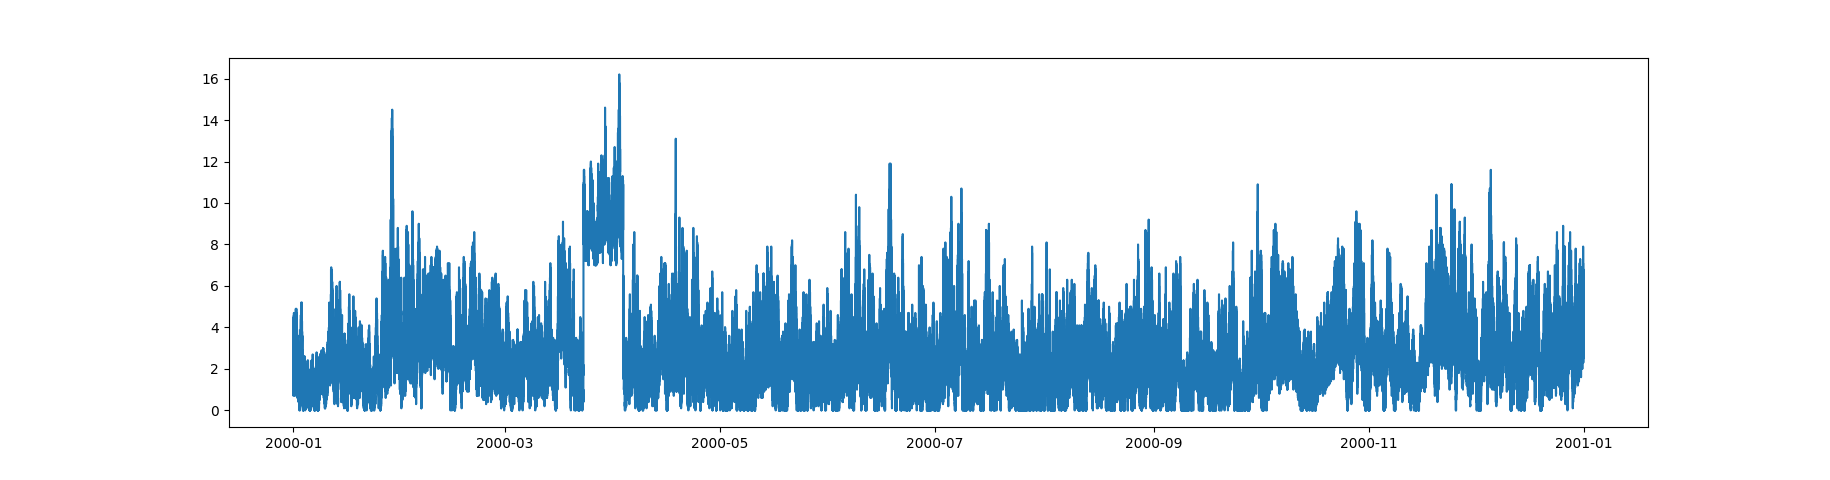
\includegraphics[width=14cm]{x1.png}
    \caption{Pirmās stacijas mērījumi}\label{fig:x1}
\end{figure}
Pirmajā stacijā marta beigās un aprīļa sākumā arī ir notikusi sensora kļūme, jo lēciens uz vērtībām, kas sākas ap 7, ir ļoti pēkšņs, un tāds pats ir arī kritiens atpakaļ. Arī pārējās stacijās šāds lēciens nav novērojams, līdz ar to varam pieņemt šo kā kļūdu, taču šos datus ir daudz grūtāk izolēt, jo katra konkrētā vērtība ir pieļaujama, tādēļ vispirms mēģināsim dziļāk analizēt datus un tikai tad apskatīsim vidējās vērtības.

% Lai arī dati katrā stacijā noteikti nav neatkarīgi viens no otra (dabas parādību novērojuma iespējamība noteikti ir atkarīga no iepriekšējās minūtes), datu ir tik daudz, ka vienkāršības labad varam pieņemt neatkarību.
Ir uzreiz skaidrs, ka novērojumi nav neatkarīgi: ja visas stacijas ir diezgan tuvu vai vērstas vienā virzienā, tad vienā un tajā pašā minūtē novērojumi, visticamāk, būs līdzīgi. Arī katrā atsevišķajā stacijā novērojumi nav neatkarīgi, jo dabas parādības notikuma iespējamība noteikti ir atkarīga no iepriekšējās minūtes, taču datu daudzums ļauj mums vispirms iztēloties, ka novērojumi ir neatkarīgi.

Tiem piemeklējot datu sadalījumu, redzam, ka dati pieņem reālas pozitīvas vērtības, un katrā stacijā gandrīz puse no mērījumiem ir starp 0 un 2, kā arī \(75\%\) mērījumu ir zem 4. Līdz ar to sadalījuma grafiks atrodas augstu starp 0 un 4, un no 500 000 mērījumiem trīs stacijās neviens nepārsniedz 16 (protams, izņemot dažus kļūdainos mērījumus). Vispārīgākais sadalījums šādam gadījumam būtu Gamma sadalījums, kuram mums jāatrod forma un mērogs. 
Diemžēl pat vienkāršam \(\Gamma(k, 1)\) sadalījumam nevar precīzi atrast aptuveno vērtību (estimator) formai \(k\), līdz ar to nāksies pieņemt formu \(k=3,5\), kurai lielākā daļa atrodas zem 4, un tad piemeklēt mērogu \(\theta=0,8\), kas augšējo asti izstiepj pareiza garuma. Kā redzams \ref{gamma}.~figūrā, kastu grafiks atbilst esošajiem datiem, tomēr mērījumu atkarība vienam no otra ir pārāk redzama \ref{fig:x1}.~figūrā, kā, piemēram, redzams, ka mērījumu vidējā vērtība gada beigās sāk pieaugt, ko ar vienkāršu Gammas sadalījumu nevar uzmodelēt.

Lai analizētu novērojumu dispersiju (variance), varam apskatīt to starpības: cik ļoti nākamais mērījums atšķiras no iepriekšējā. Tas ļauj mums atbrīvoties no vidējās vērtības līknes un apskatīt tikai dispersiju \ref{fig:starpibas}.~ figūrā. 
Varam arī ievērot to, ka starpības starp diviem mērījumiem nav neatkarīgas, jo oktobrī starpības ir pieaugušas, dati ir krasāk mainījušies, un pēc tam starpības ir arī pierimušas.

Varam ievērot divus pīķus marta beigās un aprīļa sākumā, kuros nobīdījās sensora mērījumi. Tos varam izmantot, jo tie ir lielākie pozitīvie un negatīvie lēcieni mūsu datos, un visi mērījumi starp tiem ir lielāki par 7.0, tādēļ atņemsim no šiem mērījumiem 7.0.

\begin{figure}[ht!]
    \centering
    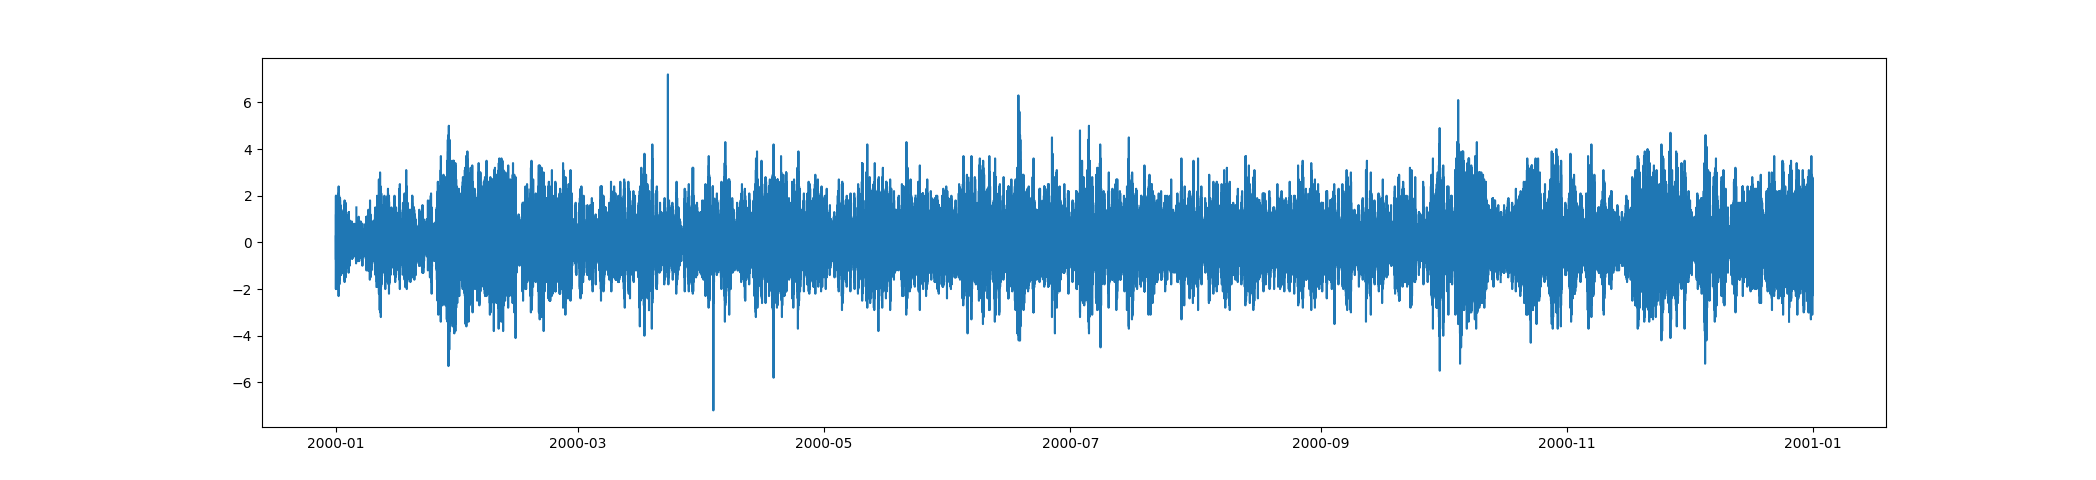
\includegraphics[width=14cm]{starpibas.png}
    \caption{Pirmās stacijas mērījumu starpības}\label{fig:starpibas}
\end{figure}


Tā kā datos vairs nav acīmredzamu kļūdu, varam aprēķināt vidējās vērtības, kas redzamas \ref{tab:videjais}.~tabulā.


\begin{table}
    \caption{Vidējās vērtības katrā stacijā pa mēnešiem}\label{tab:videjais}
    \centering
    \begin{tabular}{l|c c c}
        \toprule
        Mēnesis & \(x_1\) & \(x_2\) & \(x_3\) \\
        \midrule
        1  &  2.212  &  1.984  &  2.690 \\
        2  &  3.184  &  nan  &  3.841 \\
        3  &  2.189  &  2.335  &  2.389 \\
        4  &  2.446  &  2.703  &  2.764 \\
        5  &  1.962  &  2.080  &  2.129 \\
        6  &  2.251  &  2.147  &  2.380 \\
        7  &  2.103  &  2.025  &  2.303 \\
        8  &  2.051  &  1.944  &  2.364 \\
        9  &  1.847  &  1.821  &  2.134 \\
        10  &  2.831  &  2.881  &  3.002 \\
        11  &  3.087  &  3.111  &  3.396 \\
        12  &  2.944  &  2.974  &  3.585\\
        \bottomrule
    \end{tabular}
\end{table}



\section*{Otrais uzdevums}
Failu ielādi nācās veikt pilnīgi atšķirīgos veidos.

\begin{lstlisting}[breaklines]
Vol_URL = 'https://wis.wmo.int/operational-info/VolumeC1/VolC1.txt'
ESWI_URL = 'https://wis.wmo.int/operational-info/GTS_routeing/ESWI/ESWIroca.txt'

Vol = pd.read_csv(Vol_URL, quoting=csv.QUOTE_ALL, quotechar='"', encoding='latin-1')

if os.path.isfile('ESWIroca.txt'):
    ESWI = pd.read_csv('ESWIroca.txt')
else:
    f = open(urlretrieve(ESWI_URL)[0])
    ESWI = pd.DataFrame(columns=['TTAAii', 'CCCC', 'Receivers'])
    f.readline()
    for line in f:
        objs = line[:-1].split(',')
        objs = [item.strip('\"') for item in objs]
        sender = objs[0].split()
        ESWI = pd.concat([ESWI, pd.DataFrame([[sender[0], sender[1], objs[1:]]], columns=ESWI.columns)], ignore_index=True)
    ESWI.to_csv('ESWIroca.txt', index=False)
\end{lstlisting}
Pirmo failu \texttt{VolC1.txt} var ielādēt ļoti vienkārši, izmantojot \texttt{pandas} bibliotēku, jo tas satur tikai tabulu. Otrajā failā katrā rindiņā ir nezināms skaits elementu, līdz ar to šo failu nevar tiešā veidā pārveidot kā tabulu, taču zinām, ka pirmais elements satur \texttt{TTAAii} un \texttt{CCCC}, savukārt visi atlikušie elementi rindiņā ir ziņas saņēmēji.

Vispirms jāinicializē jauns \texttt{DataFrame} un jānolasa pirmā faila rindiņa, kas satur vienu skaitli, un tad var apskatīt katru jauno rindiņu.
Tās attiecīgi sadalot un noņemot pēdiņas, mums sanāk jauna tabula \texttt{ESWI} ar trīs kolonnām, kur trešajā atrodas saraksts (list) ar saņēmēju \texttt{CCCC} identifikatoriem.
Visbeidzot šī tabula tiek saglabāta arī lokāli, lai, atkārtoti palaižot kodu, nebūtu atkārtoti jāveic šo datu apstrāde.

\begin{figure}[ht!]
    \centering
    \includegraphics[width=13cm]{pasaule.png}
    \caption{\texttt{UMRR} ienākošo telegrammu skaits}\label{pasaule}
\end{figure}

Pielikumā~\ref{ap:II 2.a} pievienots valstu saraksts ar no tām saņemto telegrammu skaitu.
Ne visi \texttt{CCCC} kodi, kuri izsūtīja ziņas Latvijai, ir identificējami ar valsti. Attiecīgie \texttt{CCCC} kodi 
ir norādīti pielikuma beigās. Arī valstu nosaukumi ne visi bija pārveidojami par Alpha-3 kodiem, līdz ar to \ref{pasaule}.~figūra neiekļauj dažas valstis. Šo, protams, ir iespējams izlabot manuāli, taču esošā pieeja jau nešķiet optimāla, līdz ar to tas netika veikts.

Pielikumā~\ref{ap:II 3} pievienoti failu uzskaitījumi ar prasītajiem \texttt{CCCC} kodiem.

\section*{Trešais uzdevums}




\begin{figure}[ht!]
    \centering
    \includegraphics[width=13cm]{baltija.png}
    \caption{SSR Baltijā 2022-07-06}\label{baltija}
\end{figure}
\begin{figure}[ht!]
    \centering
    \includegraphics[width=7cm]{pilsetas.png}
    \caption{Stundas vidējās radiācijas vērtības Latvijas pilsētās}\label{pilsetas}
\end{figure}
Jāievēro, ka \ref{pilsetas}.~figūrā pusnakts atrodas nakts beigās. Tas liecina par to, ka laiks ir dots Griničas laika zonā, jo jūlijā Latvijā saule riet ap 22:30 un aust ap 05:30, līdz ar to saules radiācija ir ap nulli šajā laika posmā,
un pusnaktij būtu jāatrodas bez-radiācijas intervāla sākumā. Tā kā pusnakts datos atbilst Latvijas plkst.~03:00, varam datiem pieņemt Griničas laika zonu.


Attiecīgi arī \texttt{SSR} ir jāskatās trīs stundas agrāk, un \ref{baltija}.~figūrā ir izmantots lokālais, nevis Griničas laiks. Tā kā \texttt{SSR} ir summārā radiācija, tad par references laiku ir izmantota tās pašas dienas pusnakts, un attiecīgi plkst.~01:00 summārā radiācija nav būtiski palielinājusies, salīdzinot ar pusnakti.


\newpage
\appendix
\section{Uzdevums II 2.a}\label{ap:II 2.a}
\begin{multicols*}{3}
    \begin{itemize}
        \item[279] UNITED STATES OF AMERICA
\item[221] DENMARK AND FAROE ISLANDS
\item[221] RUSSIAN FEDERATION
\item[212] NORWAY
\item[189] GERMANY
\item[138] ITALY
\item[116] ANTARCTIC
\item[105] JAPAN
\item[104] TURKEY
\item[97] CANARY ISLANDS
\item[87] UNITED KINGDOM OF GREAT BRITAIN AND NORTHERN IRELAND
\item[84] SWEDEN
\item[82] CROATIA
\item[72] GREECE
\item[67] POLAND
\item[63] CZECH REPUBLIC
\item[63] MADEIRA
\item[60] SERBIA
\item[60] FINLAND
\item[54] UKRAINE
\item[53] SLOVAKIA
\item[51] BELARUS
\item[48] ICELAND
\item[48] LITHUANIA
\item[46] NETHERLANDS
\item[39] ROMANIA
\item[37] BELGIUM
\item[37] ESTONIA
\item[36] BULGARIA
\item[33] LATVIA
\item[33] CANADA
\item[32] AUSTRALIA
\item[31] IRELAND
\item[29] SWITZERLAND
\item[28] AUSTRIA
\item[26] HUNGARY
\item[26] ISRAEL
\item[23] KAZAKHSTAN
\item[22] SOUTH AFRICA (GOUGH \& MARION ISLANDS)
\item[20] EGYPT
\item[18] SLOVENIA
\item[17] MOROCCO
\item[16] TUNISIA
\item[14] BOSNIA AND HERZEGOVINA
\item[11] ARGENTINA
\item[11] GEORGIA
\item[10] HONG KONG, CHINA
\item[9] NETHERLANDS ANTILLES
\item[8] AZERBAIJAN
\item[8] REPUBLIC OF KOREA
\item[7] INDIA
\item[7] MEXICO
\item[6] NEW ZEALAND
\item[6] CYPRUS
\item[6] FIJI
\item[5] REPUBLIC OF MOLDOVA
\item[5] ALBANIA
\item[5] ARMENIA
\item[5] BRAZIL
\item[5] UZBEKISTAN
\item[4] SINGAPORE
\item[4] JORDAN
\item[4] HONDURAS
\item[3] MALTA
\item[3] NIGER
\item[3] GAMBIA
\item[3] URUGUAY
\item[3] PHILIPPINES
\item[3] SRI LANKA
\item[3] CUBA
\item[3] SAUDI ARABIA
\item[2] ETHIOPIA
\item[2] SYRIAN ARAB REPUBLIC
\item[2] VENEZUELA
\item[2] LUXEMBOURG
\item[2] RWANDA
\item[2] BOTSWANA
\item[2] MAURITIUS
\item[2] BOLIVIA
\item[2] COLOMBIA
\item[2] LEBANON
\item[2] PERU
\item[2] SUDAN
\item[1] CAYMAN ISLANDS
\item[1] TRINIDAD AND TOBAGO
\item[1] BELIZE
\item[1] DOMINICA
\item[1] KENYA
\item[1] GUATEMALA
\item[1] LIBERIA
\item[1] JAMAICA
\item[1] PANAMA
\item[1] BAHRAIN
\item[1] CHAD
\item[1] CONGO
\item[1] CHILE
\item[1] UNITED ARAB EMIRATES
\item[1] IRAN, ISLAMIC REPUBLIC OF
\item[1] CAMBODIA
\item[1] KUWAIT
\item[1] MADAGASCAR
\item[1] MALAYSIA
\item[1] MALDIVES
\item[1] NIGERIA
\item[1] NEPAL
\item[1] OMAN
\item[1] PARAGUAY
\item[1] SEYCHELLES
\item[1] TURKMENISTAN
\item[1] DEMOCRATIC REPUBLIC OF THE CONGO
\item[1] ECUADOR
\item[1] CHINA
\item[1] PAKISTAN
    \end{itemize}
\end{multicols*}

\subsection*{\texttt{CCCC} kodi bez valsts}
'LQBK', 'TFFF', 'SVVA', 'ETGG', 'LZPW', 'BIBD', 'RUSP', 'SBSL', 'SBAR', 'ZWWW', 'RUIR', 'RUAA', 'RUKG', 'SBGR', 'ZJHK', 'ZYTX', 'RURD', 'SBMQ', 'SBGL', 'SULS', 'ZUUU', 'SBCW', 'YBRF', 'LOXZ', 'SBBV', 'SACO', 'BICC', 'DAAA', 'SVMG', 'SEGU', 'SBAZ', 'EEEI', 'LOXT', 'SBCB', 'RKSI', 'ZSSS', 'SBFZ', 'SBSV', 'LZMC', 'SBCR', 'LFBD', 'VTBS', 'CWWG', 'SBSN', 'ETGT', 'LFLY', 'SBOI', 'ZBAA', 'EGJJ', 'YMRF', 'SCCI', 'OKLA', 'SAME', 'VVGL', 'CWTO', 'AGGH', 'SBPP', 'SBFI', 'RUMU', 'SCIP', 'BIIS', 'UACC', 'LFQQ', 'ZHHH', 'SAVC', 'WIII', 'SBCF', 'LFPB', 'FAOR', 'VGHS', 'RPLL', 'WAAA', 'LFST', 'SBBE', 'SUAA', 'ZGGG', 'BKPR', 'VCBI', 'SBEG', 'SCTE', 'MROC', 'RCTP', 'SBBS', 'SVMC', 'SBSG', 'SUSO', 'EPWA', 'SVBM', 'SPJC', 'VOMM', 'LTFM', 'VZIB', 'SBPJ', 'SCFA', 'SBCG', 'SBFL', 'SBMA', 'BGSF', 'LFRN', 'SBKP', 'LFML', 'VYYY', 'LTAC', 'RUSM', 'SBCT', 'BIHN', 'RUOM', 'RUMA', 'BIVM', 'YMMC', 'LROM', 'RUYK', 'ZLXY', 'CWVR', 'CIMA', 'UTTT', 'RUKR', 'SBTE', 'SBCZ', 'UATT', 'VIDP', 'SABE', 'SCEL', 'UGTB', 'LPAM', 'RUEK', 'UDYZ', 'SBCJ', 'RUMG', 'SBTT', 'SARE', 'SBRE', 'ORBI'

\subsection*{Valstis ar neatrodamiem Alpha-3 kodiem}
'TURKEY', 'DENMARK AND FAROE ISLANDS', 'ANTARCTIC', 'HONG KONG, CHINA', 'MADEIRA', 'SOUTH AFRICA (GOUGH \& MARION ISLANDS)', 'VENEZUELA', 'DEMOCRATIC REPUBLIC OF THE CONGO', 'REPUBLIC OF KOREA', 'BOLIVIA', 'NETHERLANDS ANTILLES', 'CANARY ISLANDS'

\section{Uzdevums II 3.}\label{ap:II 3}
\subsection*{Faili mapē \texttt{UMRR}}
\begin{lstlisting}[breaklines]
data/6/NORRKOPING/LATVIA/UMRR/LATVIA_ULLV10_UMRR_00.txt
data/6/NORRKOPING/LATVIA/UMRR/LATVIA_FQLV30_UMRR_XXX.txt
data/6/NORRKOPING/LATVIA/UMRR/LATVIA_ISID11_UMRR_03,09,15,21.txt
data/6/NORRKOPING/LATVIA/UMRR/LATVIA_ISCD10_UMRR_MONTHLY.txt
data/6/NORRKOPING/LATVIA/UMRR/LATVIA_SMLV10_UMRR_18.txt
data/6/NORRKOPING/LATVIA/UMRR/LATVIA_FELV40_UMRR_XXX.txt
data/6/NORRKOPING/LATVIA/UMRR/LATVIA_UKLV10_UMRR_00.txt
data/6/NORRKOPING/LATVIA/UMRR/LATVIA_UELV10_UMRR_00.txt
data/6/NORRKOPING/LATVIA/UMRR/LATVIA_ISCD60_UMRR_MONTHLY.txt
data/6/NORRKOPING/LATVIA/UMRR/LATVIA_FPLV30_UMRR_XXX.txt
data/6/NORRKOPING/LATVIA/UMRR/LATVIA_IUKD10_UMRR_00.txt
data/6/NORRKOPING/LATVIA/UMRR/LATVIA_WOLV30_UMRR_AS REQUIRED.txt
data/6/NORRKOPING/LATVIA/UMRR/LATVIA_VMLV40_UMRR_06.txt
data/6/NORRKOPING/LATVIA/UMRR/LATVIA_FPLV40_UMRR_XXX.txt
data/6/NORRKOPING/LATVIA/UMRR/LATVIA_FPLV10_UMRR_XXX.txt
data/6/NORRKOPING/LATVIA/UMRR/LATVIA_ISMD11_UMRR_00,06,12,18.txt
data/6/NORRKOPING/LATVIA/UMRR/LATVIA_USLV10_UMRR_00.txt
data/6/NORRKOPING/LATVIA/UMRR/LATVIA_SMLV10_UMRR_12.txt
data/6/NORRKOPING/LATVIA/UMRR/LATVIA_IUSD10_UMRR_00.txt
data/6/NORRKOPING/LATVIA/UMRR/LATVIA_CULV10_UMRR_MONTHLY.txt
\end{lstlisting}
\subsection*{Faili mapē \texttt{ESWI}}
\begin{lstlisting}[breaklines]
data/6/NORRKOPING/SWEDEN/ESWI/SWEDEN_WSSN31_ESWI_AS REQUIRED.txt
data/6/NORRKOPING/SWEDEN/ESWI/SWEDEN_SMVD01_ESWI_00.txt
data/6/NORRKOPING/SWEDEN/ESWI/SWEDEN_SMVA01_ESWI_18.txt
data/6/NORRKOPING/SWEDEN/ESWI/SWEDEN_IUSD15_ESWI_00,18.txt
data/6/NORRKOPING/SWEDEN/ESWI/SWEDEN_SMVF01_ESWI_18.txt
data/6/NORRKOPING/SWEDEN/ESWI/SWEDEN_IUKN41_ESWI_00,06,12,18.txt
data/6/NORRKOPING/SWEDEN/ESWI/SWEDEN_SMVB01_ESWI_18.txt
data/6/NORRKOPING/SWEDEN/ESWI/SWEDEN_SMVD01_ESWI_06.txt
data/6/NORRKOPING/SWEDEN/ESWI/SWEDEN_SMVD01_ESWI_12.txt
data/6/NORRKOPING/SWEDEN/ESWI/SWEDEN_ISMD61_ESWI_00,06,12,18.txt
data/6/NORRKOPING/SWEDEN/ESWI/SWEDEN_SASN33_ESWI_H+20,H+50.txt
data/6/NORRKOPING/SWEDEN/ESWI/SWEDEN_IUXD13_ESWI_00,12.txt
data/6/NORRKOPING/SWEDEN/ESWI/SWEDEN_IUKD11_ESWI_00.txt
data/6/NORRKOPING/SWEDEN/ESWI/SWEDEN_SIVA21_ESWI_09.txt
data/6/NORRKOPING/SWEDEN/ESWI/SWEDEN_SIVA21_ESWI_21.txt
data/6/NORRKOPING/SWEDEN/ESWI/SWEDEN_IUKD15_ESWI_00,18.txt
data/6/NORRKOPING/SWEDEN/ESWI/SWEDEN_SIVF21_ESWI_09.txt
data/6/NORRKOPING/SWEDEN/ESWI/SWEDEN_SIVF21_ESWI_21.txt
data/6/NORRKOPING/SWEDEN/ESWI/SWEDEN_WVSN31_ESWI_AS REQUIRED.txt
data/6/NORRKOPING/SWEDEN/ESWI/SWEDEN_SIVD21_ESWI_03.txt
data/6/NORRKOPING/SWEDEN/ESWI/SWEDEN_SIVB21_ESWI_21.txt
data/6/NORRKOPING/SWEDEN/ESWI/SWEDEN_SIVB21_ESWI_09.txt
data/6/NORRKOPING/SWEDEN/ESWI/SWEDEN_UASN61_ESWI_AS REQUIRED.txt
data/6/NORRKOPING/SWEDEN/ESWI/SWEDEN_IUKD01_ESWI_00.txt
data/6/NORRKOPING/SWEDEN/ESWI/SWEDEN_SIVD21_ESWI_15.txt
data/6/NORRKOPING/SWEDEN/ESWI/SWEDEN_IUSD16_ESWI_00,12.txt
data/6/NORRKOPING/SWEDEN/ESWI/SWEDEN_SNSN86_ESWI_01, 02, 04, 05, 07, 08, 10, 11, 13, 14, 16, 17, 19, 20 ,22, 23.txt
data/6/NORRKOPING/SWEDEN/ESWI/SWEDEN_ISND61_ESWI_01,02,04,05,07,08,10,11,13,14,16,17,19,20,22,23.txt
data/6/NORRKOPING/SWEDEN/ESWI/SWEDEN_SIVA21_ESWI_03.txt
data/6/NORRKOPING/SWEDEN/ESWI/SWEDEN_SIVA21_ESWI_15.txt
data/6/NORRKOPING/SWEDEN/ESWI/SWEDEN_IUKD06_ESWI_00,12.txt
data/6/NORRKOPING/SWEDEN/ESWI/SWEDEN_SASN31_ESWI_H+20,H+50.txt
data/6/NORRKOPING/SWEDEN/ESWI/SWEDEN_FTSN31_ESWI_05,11,17,23.txt
data/6/NORRKOPING/SWEDEN/ESWI/SWEDEN_SIVB21_ESWI_15.txt
data/6/NORRKOPING/SWEDEN/ESWI/SWEDEN_FCSN31_ESWI_02,05,08,11,14,17,23.txt
data/6/NORRKOPING/SWEDEN/ESWI/SWEDEN_SIVF21_ESWI_15.txt
data/6/NORRKOPING/SWEDEN/ESWI/SWEDEN_ISID61_ESWI_03,09,15,21.txt
data/6/NORRKOPING/SWEDEN/ESWI/SWEDEN_SIVF21_ESWI_03.txt
data/6/NORRKOPING/SWEDEN/ESWI/SWEDEN_SIVD21_ESWI_09.txt
data/6/NORRKOPING/SWEDEN/ESWI/SWEDEN_SIVD21_ESWI_21.txt
data/6/NORRKOPING/SWEDEN/ESWI/SWEDEN_SIVB21_ESWI_03.txt
data/6/NORRKOPING/SWEDEN/ESWI/SWEDEN_WOSN42_ESWI_XXX.txt
data/6/NORRKOPING/SWEDEN/ESWI/SWEDEN_SMVA01_ESWI_06.txt
data/6/NORRKOPING/SWEDEN/ESWI/SWEDEN_SMVA01_ESWI_12.txt
data/6/NORRKOPING/SWEDEN/ESWI/SWEDEN_SMVF01_ESWI_00.txt
data/6/NORRKOPING/SWEDEN/ESWI/SWEDEN_IUSD01_ESWI_00.txt
data/6/NORRKOPING/SWEDEN/ESWI/SWEDEN_SMVB01_ESWI_00.txt
data/6/NORRKOPING/SWEDEN/ESWI/SWEDEN_STSN42_ESWI_XXX.txt
data/6/NORRKOPING/SWEDEN/ESWI/SWEDEN_IUSN41_ESWI_00,06,12,18.txt
data/6/NORRKOPING/SWEDEN/ESWI/SWEDEN_UASN71_ESWI_AS REQUIRED.txt
data/6/NORRKOPING/SWEDEN/ESWI/SWEDEN_IUSD06_ESWI_00,12.txt
data/6/NORRKOPING/SWEDEN/ESWI/SWEDEN_SMVA01_ESWI_00.txt
data/6/NORRKOPING/SWEDEN/ESWI/SWEDEN_ISND22_ESWI_01,02,04,05,07,08,10,11,13,14,16,17,19,20,22,23.txt
data/6/NORRKOPING/SWEDEN/ESWI/SWEDEN_FQSN40_ESWI_XXX.txt
data/6/NORRKOPING/SWEDEN/ESWI/SWEDEN_STSN43_ESWI_XXX.txt
data/6/NORRKOPING/SWEDEN/ESWI/SWEDEN_SMVF01_ESWI_06.txt
data/6/NORRKOPING/SWEDEN/ESWI/SWEDEN_SMVF01_ESWI_12.txt
data/6/NORRKOPING/SWEDEN/ESWI/SWEDEN_ISCD01_ESWI_MONTHLY.txt
data/6/NORRKOPING/SWEDEN/ESWI/SWEDEN_IUSD11_ESWI_00.txt
data/6/NORRKOPING/SWEDEN/ESWI/SWEDEN_SMVB01_ESWI_06.txt
data/6/NORRKOPING/SWEDEN/ESWI/SWEDEN_SMVB01_ESWI_12.txt
data/6/NORRKOPING/SWEDEN/ESWI/SWEDEN_IUKD16_ESWI_00,12.txt
data/6/NORRKOPING/SWEDEN/ESWI/SWEDEN_SMVD01_ESWI_18.txt
\end{lstlisting}
\subsection*{Faili mapē \texttt{EEMH}}
\begin{lstlisting}[breaklines]
data/6/NORRKOPING/ESTONIA/EEMH/ESTONIA_STEO11_EEMH_XXX.txt
data/6/NORRKOPING/ESTONIA/EEMH/ESTONIA_FEEO40_EEMH_XXX.txt
data/6/NORRKOPING/ESTONIA/EEMH/ESTONIA_SIEO40_EEMH_15.txt
data/6/NORRKOPING/ESTONIA/EEMH/ESTONIA_SMEO41_EEMH_06.txt
data/6/NORRKOPING/ESTONIA/EEMH/ESTONIA_SMEO41_EEMH_12.txt
data/6/NORRKOPING/ESTONIA/EEMH/ESTONIA_ISND21_EEMH_01,02,04,05,07,08,10,11,13,14,16,17,19,20,22,23.txt
data/6/NORRKOPING/ESTONIA/EEMH/ESTONIA_SIEO40_EEMH_03.txt
data/6/NORRKOPING/ESTONIA/EEMH/ESTONIA_IUXD11_EEMH_00.txt
data/6/NORRKOPING/ESTONIA/EEMH/ESTONIA_SNEO41_EEMH_01,02,04,05,07,08,10,11,13,14,16,17,19,20,22,23.txt
data/6/NORRKOPING/ESTONIA/EEMH/ESTONIA_SIEO20_EEMH_15.txt
data/6/NORRKOPING/ESTONIA/EEMH/ESTONIA_ISAD30_EEMH_EVERY 10 MINUTES.txt
data/6/NORRKOPING/ESTONIA/EEMH/ESTONIA_STEO10_EEMH_XXX.txt
data/6/NORRKOPING/ESTONIA/EEMH/ESTONIA_SMEO41_EEMH_00.txt
data/6/NORRKOPING/ESTONIA/EEMH/ESTONIA_FQEO30_EEMH_XXX.txt
data/6/NORRKOPING/ESTONIA/EEMH/ESTONIA_SIEO20_EEMH_03.txt
data/6/NORRKOPING/ESTONIA/EEMH/ESTONIA_SNEO40_EEMH_01,02,04,05,07,08,10,11,13,14,16,17,19,20,22,23.txt
data/6/NORRKOPING/ESTONIA/EEMH/ESTONIA_FPEO40_EEMH_XXX.txt
data/6/NORRKOPING/ESTONIA/EEMH/ESTONIA_SMEO10_EEMH_12.txt
data/6/NORRKOPING/ESTONIA/EEMH/ESTONIA_SMEO10_EEMH_06.txt
data/6/NORRKOPING/ESTONIA/EEMH/ESTONIA_USEO10_EEMH_00.txt
data/6/NORRKOPING/ESTONIA/EEMH/ESTONIA_IUSD11_EEMH_00.txt
data/6/NORRKOPING/ESTONIA/EEMH/ESTONIA_SMEO40_EEMH_18.txt
data/6/NORRKOPING/ESTONIA/EEMH/ESTONIA_VMEO40_EEMH_XXX.txt
data/6/NORRKOPING/ESTONIA/EEMH/ESTONIA_ISMD40_EEMH_00,06,12,18.txt
data/6/NORRKOPING/ESTONIA/EEMH/ESTONIA_SMEO10_EEMH_00.txt
data/6/NORRKOPING/ESTONIA/EEMH/ESTONIA_IUKD10_EEMH_00.txt
data/6/NORRKOPING/ESTONIA/EEMH/ESTONIA_SIEO41_EEMH_21.txt
data/6/NORRKOPING/ESTONIA/EEMH/ESTONIA_SIEO41_EEMH_09.txt
data/6/NORRKOPING/ESTONIA/EEMH/ESTONIA_SUEO40_EEMH_XXX.txt
data/6/NORRKOPING/ESTONIA/EEMH/ESTONIA_SMEO10_EEMH_18.txt
data/6/NORRKOPING/ESTONIA/EEMH/ESTONIA_FPEO43_EEMH_XXX.txt
data/6/NORRKOPING/ESTONIA/EEMH/ESTONIA_UKEO10_EEMH_00.txt
data/6/NORRKOPING/ESTONIA/EEMH/ESTONIA_SNEO21_EEMH_01,02,04,05,07,08,10,11,13,14,16,17,19,20,22,23.txt
data/6/NORRKOPING/ESTONIA/EEMH/ESTONIA_ISCD60_EEMH_MONTHLY.txt
data/6/NORRKOPING/ESTONIA/EEMH/ESTONIA_SMEO40_EEMH_00.txt
data/6/NORRKOPING/ESTONIA/EEMH/ESTONIA_ISID20_EEMH_03,09,15,21.txt
data/6/NORRKOPING/ESTONIA/EEMH/ESTONIA_ISXD64_EEMH_DAILY.txt
data/6/NORRKOPING/ESTONIA/EEMH/ESTONIA_ISMD10_EEMH_00,06,12,18.txt
data/6/NORRKOPING/ESTONIA/EEMH/ESTONIA_SIEO41_EEMH_03.txt
data/6/NORRKOPING/ESTONIA/EEMH/ESTONIA_ULEO10_EEMH_00.txt
data/6/NORRKOPING/ESTONIA/EEMH/ESTONIA_SIEO41_EEMH_15.txt
data/6/NORRKOPING/ESTONIA/EEMH/ESTONIA_CSEO10_EEMH_MONTHLY.txt
data/6/NORRKOPING/ESTONIA/EEMH/ESTONIA_SMEO40_EEMH_12.txt
data/6/NORRKOPING/ESTONIA/EEMH/ESTONIA_SMEO40_EEMH_06.txt
data/6/NORRKOPING/ESTONIA/EEMH/ESTONIA_IUKD11_EEMH_00.txt
data/6/NORRKOPING/ESTONIA/EEMH/ESTONIA_SIEO40_EEMH_09.txt
data/6/NORRKOPING/ESTONIA/EEMH/ESTONIA_SIEO40_EEMH_21.txt
data/6/NORRKOPING/ESTONIA/EEMH/ESTONIA_ISCD10_EEMH_MONTHLY.txt
data/6/NORRKOPING/ESTONIA/EEMH/ESTONIA_IUSD10_EEMH_00.txt
data/6/NORRKOPING/ESTONIA/EEMH/ESTONIA_ISND40_EEMH_01,02,04,05,07,08,10,11,13,14,16,17,19,20,22,23.txt
data/6/NORRKOPING/ESTONIA/EEMH/ESTONIA_SMEO41_EEMH_18.txt
data/6/NORRKOPING/ESTONIA/EEMH/ESTONIA_ISID40_EEMH_03,09,15,21.txt
data/6/NORRKOPING/ESTONIA/EEMH/ESTONIA_WOEO30_EEMH_XXX.txt
data/6/NORRKOPING/ESTONIA/EEMH/ESTONIA_SIEO20_EEMH_09.txt
data/6/NORRKOPING/ESTONIA/EEMH/ESTONIA_SIEO20_EEMH_21.txt
data/6/NORRKOPING/ESTONIA/EEMH/ESTONIA_UEEO10_EEMH_00.txt
\end{lstlisting}




\end{document}